
\chapter{\listfigurename}

\begin{lof}

\item[封面及篇头扉页]两个“三字件”(“GEB—集异璧”和“EGB—异集璧”)悬在空中,在室内三个相交汇的平面上投出字母—汉字状的影子。“三字件”是指那两个造型奇特的木块,它们的形状使得它们在三个互相垂直的方向上的投影是三个不同的符号。作者为了将哥德尔(G)、艾舍尔(E)和巴赫(B)的名字编织到一个醒目的图案中去曾煞费苦心,一天晚上,他忽然灵机一动,产生了“三字件”这个设想(当然,他的三字件只涉及英文字母)。于是,他使用带锯和尖钻铣刀加工了两个边长4英寸的红木块,并用照相机在适当的光线下拍摄了下来(见封面)。中译本的此图保留了作者的构思,但在英文字母里嵌进了谐音的汉字,并使二者互为衬底(见上、下篇的篇头扉页)。因此这幅图(以及上、下篇的篇名本身)也成了一种“翻译”。与原作不同的是,“译图”不是实物照片,而是刘皓明手绘的。

\item[本目录之后]用古希伯来文写的《创世纪》的开头。

\listoffigures

\end{lof}

\bigskip

\begin{center}
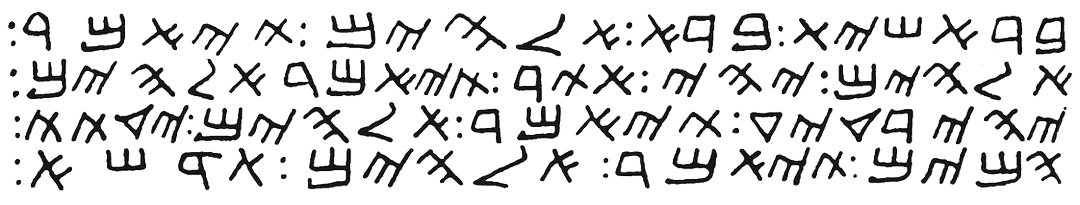
\includegraphics{img_lof.png}
\end{center}
